\chapter{DUyxrara mAyAcwkada visheVSate}

\begin{center}
\begin{tabular}{|>{$}c<{$}|>{$}c<{$}|>{$}c<{$}|>{$}c<{$}|}
\hline
16 & 3 & 2 & 13\\
\hline
5 & 10 & 11 & 8\\
\hline
9 & 6 & 7 & 12\\
\hline
4 & 15 & 14 & 1\\
\hline
\end{tabular}
\end{center}
meVle barediruva {\rm 16} maneya oMdu mAyAcwkavanunx racisidavaru yAreMdu sariyAgi tiLidilalx. idu modalu kaMDu baMdadudx samAdhiyoMdara sAmxraka shileya meVle DUyxrarf eMbuvanu {\rm 1514} ralilx idanunx baredaneMdu UhisalAgide. I mAyAcwka aMdiniMda Atana hesarinalelxV hesaruvAsiyAgide.

I mAyAcwkada visheVSate eMdare.
\begin{enumerate}
\item[{\rm 1)}] parxtiyoMdu aDaDxsAlina saMKeyxgaLa motatx {\rm 34}
\begin{align*}
16+3+2+13 &=34\\
5+10+11+8 &=34\\
9+6+7+12 & =34\\
4+15+14=1 &=34
\end{align*}

\item[{\rm 2)}] parxtiyoMdu kaMbasAlina saMKeyxgaLa motatx {\rm 34}
\begin{align*}
16+5+9+4 &=34\\
3+10+6+15 &=34\\
2+11+7+14 & =34\\
13+8+12+1 &=34
\end{align*}

\item[{\rm 3)}] eDaBAgadiMda meVliMda keLakekx kaNaR saKeyxgaLa motatx {\rm 34}
$$
16+10+7+1=34
$$

\item[{\rm 4)}] balaBAgadiMda meVliMda keLakekx kaNaRsaMKeyxgaLa motatx {\rm 34}
$$
13+11+6+4 =34
$$

\item[{\rm 5)}] eDaBAgadiMda keLaginiMda meVlkekx kaNaRsaMKeyxgaLa motatx {\rm 34}
$$
4+6+11+13=34
$$

\item[{\rm 6)}] balaBAgadiMda, keLaginiMda meVlakekx kaNaRsaMKeyxgaLa motatx {\rm 34}
$$
1+7+10+16=34
$$

\item[{\rm 7)}] mAyAcwkada mUlegaLalilxruva saMKeyxgaLa motatx {\rm 34}
$$
16+4+1+13=34
$$ 

\item[{\rm 8)}] {\rm 16} manegaLiruva I cwkadalilx {\rm 4} manegaLuLaLx {\rm 4} cwkagaLive parxtiyoMdu {\rm 4} manegaLa oMdoMdu cwkavU {\rm 34} kekx sama
\begin{align*}
16+3+5+10 &=34\\
2+13+11+8 &=34\\
9+6+4+15 & =34\\
7+12+14+1 &=34
\end{align*}

\item[{\rm 9)}] DUyxrarana mAyAcwka samamitige oMdu oLeLxya udAharaNe
\begin{figure}[H]
\centering
\includegraphics[scale=.8]{src/figures/m_121.eps}
\end{figure}

\begin{align*}
3+5+14+12 &=34\\
2+8+15+9  &=34
\end{align*}

\item[{\rm 10)}] aSeTxV alalx meVle barediruva saMKeyxgaLa vagaRgaLa motatxvU sama
\begin{align*}
3^2+5^2+14^2+12^2 &=374\\
2^2+8^2+15^2+9^2 &=374
\end{align*}

\item[{\rm 11)}] matotxMdu visheVSa meVle barediruva saMKeyxgaLa GanagaLa motatxvU sama
\begin{align*}
3^3+5^3+14^3+12^3 &=4624\\
2^3+8^3+15^3+9^3 &=4624
\end{align*}

\item[{\rm 12)}] mAyAcwkada meVlineraDu aDaDxsAlugaLalilxruva saMKeyxgaLa vagaRgaLa motatxvu keLagina eraDu aDaDxsAlugaLalilxruva saMKeyxgaLa vagaRgaLa motatxkekx sama.
\begin{align*}
16^2+3^2+2^2+13^2+5^2+10^2+11^2+8^2 &=748\\
9^2+6^2+7^2+12^2+4^2+15^2+14^2+1^2 &=748
\end{align*}

\item[{\rm 13)}] mAyAcwkada modalina eraDu kaMba sAlugaLalilxruva saMKeyxgaLa vagaRgaLa motatxvu koneya eraDu kaMba sAlugaLalilxruva saMKeyxgaLa vagaRgaLa motatxkekx sama.
\begin{align*}
16^2+5^2+9^2+4^2+3^2+10^2+6^2+15^2 &=748\\
2^2+11^2+7^2+14^2+13^2+6^2+12^2+1^2 &=748
\end{align*}

\item[{\rm 14)}] mAyAcwkada oMdu matutx mUraneya (payARya) aDaDxsAlugaLalilxruva saMKeyxgaLa vagaRgaLa motatxvu, eraDu matutx nAlakxneya (payARya) aDaDxsAlugaLalilxruva saMKeyxgaLa vagaRgaLa motatxkekx sama.
\begin{align*}
16^2+3^2+2^2+13^2+9^2+6^2+7^2+12^2 &=748\\
5^2+10^2+11^2+8^2+4^2+15^2+14^2+1^2 &=748
\end{align*}

\item[{\rm 15)}] mAyAcwkada oMdu matutx mUraneya (payARya) kaMba sAlugaLalilx iruva saMKeyxgaLa vagaRgaLa motatxvu eraDu matutx nAlakxneya (payARya) kaMba sAlugaLalilxruva saMKeyxgaLa vagaRgaLa motatxkekx sama.
\begin{align*}
16^2+5^2+9^2+4^2+2^2+11^2+7^2+14^2 &=748\\
3^2+10^2+6^2+15^2+13^2+8^2+12^2+1^2 &=748
\end{align*}

\item[{\rm 16)}] I mAyAcwkada madhayxdalilxruva reVKeya eDabalabadiyalilx keVMdarxdiMda sama pAshavxRte hoMdiruva manegaLalilxna saMKeyxgaLa motatx {\rm 17} kekx sama.
\begin{gather*}
16+1=17, \quad 13+4=17, \quad 10+7=17, \quad 6+11=17 \\
2+15=17, \quad 3+14=17.
\end{gather*}
 
\item[{\rm 17)}] I mAyAcwkada madhayxdalilxruva {\rm 4} manegaLa motatxvU {\rm 34}
$$
10+11+6+7=34
$$

\item[{\rm 18)}] I mAyAcwkada {\rm 4} mUlegaLalilxruva saMKeyxgaLa motatxvU {\rm 34}
$$
16+13+4+1=34
$$
\end{enumerate}

DUyxrarana mAyAcwkada {\rm 4} mUlegaLalilxruva saMKeyxgaLanunx adalu badalu mADidarU modalinaMteyeV. aDaDxsAlu, kaNaRgaLa motatx madhayxda eraDu kaMbasAlugaLa motatx {\rm 34} Agirutatxde.
\begin{figure}[H]
\centering
\includegraphics[scale=.8]{src/figures/m_123.eps}
\end{figure}


\begin{alignat*}{3}
\text{\bf aDaDxsAlu }\qquad  && 13+3+2+16&&=34\\
&&5+10+11+8&&=34\\
&&9+6+7+12&&=34\\
&&1+15+14+4&&=34\\[0.2cm]
\text{\bf kaMbasAlu} \qquad  &&13+10+7+4 &&=34\\
&&1+6+11+16&&=34
\end{alignat*}

cwkada {\rm 4} mUle saMKeyxgaLa motatxvU {\rm 34}
$$
13+16+1+4=34
$$

mUlemUle saMKeyxgaLa motatxvU sama $13+4=17$, \quad $16+1=17$

DUyxrarana mAyA cwkadalilxruva eraDu matutx mUraneV kaMba sAlugaLanunx adalu badalu mADidarU modalinaMteyeV aDaDxsAlu, kaMbasAlu matutx kaNaRgaLa motatx {\rm 34} kekxV Agirutatxde.

\begin{figure}[H]
\centering
\includegraphics[scale=.8]{src/figures/m_125.eps}
\end{figure}

\begin{alignat*}{3}
\text{\bf aDaDxsAlu }\qquad  && 16+2+3+13&&=34\\
&&5+11+10+8&&=34\\
&&9+7+6+12&&=34\\
&&4+14+15+1&&=34\\[0.2cm]
\text{\bf kaMbasAlu} \qquad  &&16+5+9+4 &&=34\\
&&2+11+7+14&&=34\\
&&3+10+6+15&&=34\\
&&13+8+12+1&&=34\\[0.2cm]
\text{\bf kaNaR} \qquad  &&4+7+10+13 &&=34\\
&&16+11+6+1&&=34\\
\end{alignat*}
